% 默认单面打印 oneside 、硕士论文模板 master

\documentclass[oneside, master,normal]{BIT-thesis-grd-jdh}

% 模板选项: 硕士论文 master; 博士论文 doctor
% 正常模式:normal  自查重模式:selfSimilarCheck  盲审模式:blindCheck
% 提交学校的查重文件可以直接使用normal模式结果
% 自查重模式主要用于关闭图片、公式等内容的显示,以减少文章字符数和降低PDF转word过程中出现的乱码,节省查重费用支出。应结合\insertcontents系列命令使用。对于土豪此选项没有任何卵用。。。。。
% 盲审模式主要根据盲审文件格式要求,隐去了作者、导师、致谢等信息,更改发表论文的格式


\begin{document}

%%%%%%%%%%%%%%%%%%%%%%%%%%%%%%
%% 封面
%%%%%%%%%%%%%%%%%%%%%%%%%%%%%%

% 中文封面内容(关注内容而不是表现形式)
\classification{TQ028.1} %可参考http://www.clcindex.com/category/TN91/
\UDC{540}

\title{这是一个有英文单词RapidIO的论文标题}
\vtitle{这是一个有英文单词\makeVerticalenWords{RapidIO}的竖排标题}
\author{张三}
\institute{信息与电子学院}
\advisor{**教授}
\chairman{**教授}
\degree{工学硕士(博士)}
\major{电子科学与技术}
\school{北京理工大学}
\defenddate{2019年6月}
%\studentnumber{**********}


% 英文封面内容(关注内容而不是表现形式)
\englishtitle{A Thesis Title with English word RapidIO}
\englishauthor{Zhangsan}
\englishadvisor{Prof. **}
\englishchairman{Prof. **}
\englishschool{Beijing Insititute of Technology}
\englishinstitute{School of Information and Electronics}
\englishdegree{Master}
\englishmajor{Electronics Science and Technology}
\englishdate{6,2019}

% 封面绘制
\maketitle

% 中文信息
\makeChineseInfo

% 英文信息
\makeEnglishInfo

%打印竖排论文题目
\makeVerticalTitle

% 论文原创性声明和使用授权
\makeDeclareOriginal

%%%%%%%%%%%%%%%%%%%%%%%%%%%%%%
%% 前置部分
%%%%%%%%%%%%%%%%%%%%%%%%%%%%%%
\frontmatter

% 摘要
%%==================================================
%% abstract.tex for BIT Master Thesis
%% modified by Xinting Xu
%% version: 0.1
%% last update: 2020-03-06
%%==================================================

\begin{abstract}
%本文的主要研究工作,是在VoLTE场景下,通过主动丢包的方式,构造安全、鲁棒的时间隐通道。伴随着第4代通信技术的应用,基于数据包交换的VoLTE(Voice over LTE)技术,取代了基于电路交换的传统通话技术。得益于LTE网络的高带宽、流量细分能力,VoLTE不仅为用户提供了低延迟、高清晰度的语音通话,也将低延迟的视频通话变为可能。
%借助实时传输协议RTP(Real-time Transport Protocol),VoLTE音视频数据被切分为独立的流,利用数据包优先级的差异,在保证传输效果的同时,提高抗干扰能力。对于语音数据流来说,基带内集成的信号采集单元,直接将编码后的数据打包为RTP数据包,经LTE组件发送到基站进行传输。另一方面,视频数据的来源是智能终端的摄像头模块,需要由应用处理器完成图像信息采集、压缩、编码,并按照RTP格式进行打包,最终交付基带处理器进行发送。

%由于处理途径及优先级方面的差异,数量较少的语音数据包,能够保持稳定且低丢包率的传输效果;而数量众多的视频数据包,受空口噪声的干扰,产生丢包现象不可避免。另一方面,VoLTE的通话双方均为无线终端,两侧的噪声强度和干扰阶段是不同的,丢包事件可能发生于任意一方、任意阶段,对用户来说,无法区分产生丢包的实际位置。因此,通过丢弃具有特定数据包序号的数据包,构造时间隐通道的设计方案,符合实际应用场景的约束,具有可行性。

%通过分析VoLTE视频流及语音流特征,结合实际通话测试结果,选择VoLTE视频流作为隐蔽消息的传输载体。经过统计分析,VoLTE丢包的主要类型为离散的丢包事件,并夹杂随机长度的连续丢包事件。类比时间隐通道的分析方法,对VoLTE丢包特征的分析,由分布统计和分布一致性检验两个维度组成。通过统计视频数据包在IPD(inter-packet delay)、突发丢包长度、窗口内丢包数量的分布情况,得到对应的分布特征。对独立的分布特征进行对比,即可得到不同视频流之间的差异,通过多维度的分析检测,对时间隐通道的抗检测性能力的提升,有重要的参考价值。

%基于Zig-Zag矩阵的时间隐通道方案,将原始的隐蔽消息,嵌入到各个数据包区间的丢包位置中,并引入HASH校验算法,提高传输过程的鲁棒性。对于待发送的隐蔽消息,按照设定的参数,首先切分为固定长度的消息块。接下来,为每一个数据块生成同等长度的校验块。然后按照设定的Zig-Zag矩阵,将消息块及校验块映射到消息符号,也就是数据包序号的相对偏移量。最后,将消息符号转换为数据包序号,并在发送队列中进行剔除。通过添加额外的校验块,解调过程中降低网络噪声的干扰;经过Zig-Zag矩阵的逆映射,噪声中的连续丢包被映射到离散的消息值,结合校验块完成去噪过程;调整传输参数后,该方案能够通过常用的抗检测性方案。

%基于多重HASH校验的时间隐通道方案,通过添加多重校验块、采用自校验的映射矩阵,在保证抗检测性的基础上,进一步提高了鲁棒性。隐蔽消息按照设定的参数,切分为定长消息块,接下来基于HASH的组间校验块被拼接到消息块末尾。接下来,在每个消息块及校验块组合的基础上,拼接基于CRC的自校验块,构成码字。根据码字的字长,码字被转换为代表组内序号的符号,并为每一组符号添加随机偏移量。最后,参照映射矩阵的定义,将符号映射为相对偏移量,最终转换为数据包序号。在发送队列中,将具有目标序号的数据包丢弃,调制过程完成。通过进行抗检测性测试、鲁棒性测试及性能测试,该时间隐通道方案具有充分的网络适应能力,在各方面的表现达到隐通道的基本要求。

%修改为以下表述方式
时间隐通道是一个经典的研究问题,对。。。事关重要。

VoLTE是一种新型的网络环境,采用了新的设计,原有的隐通道存在不适应的问题。

本文提出了解决方案,解决了该问题。本文针对VoLTE时间隐通道检测方法、基于Zigzag矩阵的时间隐通道构造方法、基于多重校验的时间隐通道构造方法四个方面展开研究。

\begin{itemize}
\item 提出了一种VoLTE环境下,对基于主动丢包的时间隐通道的检测方法。利用……方法,实现了对……的检测。实验结果分析表明,……是有效可行的。

\item 提出了一种基于Zigzag矩阵的时间隐通道构造方法。通过……处理方法,结合……,实现了鲁棒性好,抗检测能力强的时间隐通道构造方法。实验结果分析表明,该方法可以实现误码率低于……,传输性能不低于……。

\item 提出了一种基于多重校验的时间隐通道构造方法。通过添加组间校验、码字自校验及映射矩阵的校验,有效保证了传输过程的鲁棒性。实验结果分析表明,该方法可以实现误码率低于……,传输性能不低于……。
\end{itemize}

\keywords{时间隐通道; VoLTE; 主动丢包; 鲁棒性; 抗检测性}
\end{abstract}

\begin{englishabstract}

   In order to exploit …….
   
\englishkeywords{Covert Timing Channel; VoLTE; Packet Dropout; Robustness; Undetectability}

\end{englishabstract}

%% 符号对照表,可选,如不用可注释掉
\begin{denotation}
	
\item[VoLTE] Voice over LTE,基于LTE的音视频通话技术
\item[CTC] Covert Timing Channel,时间隐通道
\item[RTP] Real-time Transport Protocol,实时传输协议
\item[UDP] User Datagram Protocol,用户数据包协议
\item[HASH] HASH信息摘要算法
\item[CRC] Cyclic Redundancy Check,循环冗余校验码
\item[IPD] Inter-Packet Delay,数据包时间间隔
\item[] 
\item[$C_{i}$] 第i个码字,消息及校验信息组成的二进制数据
\item[$S_{j}$] 第j个符号,可观测的丢包相对位置
\item[$BL$] Block Length的缩写,消息块的二进制位数
\item[$L_{Codeword}$] 码字Codeword的二进制位数
\item[$L_{HASH}$] 嵌入在Codeword中的HASH校验块位数
\item[$L_{CRC}$] 嵌入在Codeword中的CRC校验块位数
\item[$R$] 码字组间校验关系的复位周期
\item[$M_{cols}$] 码字与符号映射矩阵的列数
\item[$M_{rows}$] 码字与符号映射矩阵的行数
\item[\textit{\textbf{M}}] 码字与符号的映射矩阵
\item[$\textit{\textbf{M}}_{row,\ col}$] 映射矩阵中的第$row$行第$col$列的元素
\item[] 
\item[K-S检验] Kolmogorov-Smirnov检验
\item[K-L散度] Kullback-Leibler divergence
\item[CDF] Cumulative Distribution Function,累积分布函数
\item[PMF] Probability Mass Function,概率质量函数

\end{denotation}

% 加入目录
\tableofcontents


%加入图、表索引(同时取消图表索引中章之间的垂直间隔)
%硕士论文貌似不做硬性要求,可不加
\let\origaddvspace\addvspace
\renewcommand{\addvspace}[1]{}
\listoffigures
\listoftables
\renewcommand{\addvspace}[1]{\origaddvspace{#1}}



%%%%%%%%%%%%%%%%%%%%%%%%%%%%%%
%% 正主体部分
%%%%%%%%%%%%%%%%%%%%%%%%%%%%%%
\mainmatter

%% 各章正文内容
%\chapter{引言}
\label{chap:intro}
%在下方加入各小节内容
\section{研究背景和意义}
\label{sec:intro:backgroud}

%介绍什么是隐通道

%传统的时间隐通道,是利用数据的时间变化特性,承载目标数据。例如基于IP的时间隐通道(IP-CTC)[3].,基于回复时间的隐通道(TR-CTC)[4].,基于IPD的时间隐通道(IPD-CTC),利用数据包的长度变化规律来传送数据[10].,利用数据包之间的时间间隔(IPD)传送数据[12].,或者基于数据包分类的时间隐通道[13].,以及基于模型的时间隐通道(MB-CTC)[11].。

隐通道的明确定义,由Lampson在1973年提出\nupcite{4317620},隐通道能够打破系统中的安全限制,实现消息在不同安全级别之间的隐蔽传输。隐通道的存在意义,是在传输信道被监听的前提下,实现数据传输过程,并且监听者无法察觉传输过程。监听者通常对数据内容及传输过程进行监控,只允许传输符合规则的数据,拦截其它的会话请求。研究VoLTE中的时间隐通道构建方法,解决当双方只被允许进行VoLTE通话时,数据隐蔽、鲁棒传输的需求。

经过研究探索,随着互联网应用范围的扩大,网络应用逐渐丰富,隐通道的应用环境由传统的单主机平台,扩展到各种类型的网络设备之中。
隐通道的实现方式多种多样,根据构建方式的差异,隐通道通常被划分为时间隐通道及存储隐通道两种类型,存储隐通道依赖于双方对相同存储位置的读写访问,时间隐通道依赖于双方对时间特征的识别。\nupcite{1702197}
随着移动互联网的不断扩展,隐通道为终端之间的安全隐蔽传输,提供了可行的解决方案,满足了特定需求场景下的传输需求。\nupcite{6542541}

\insertFigure{
	\begin{figure}
	    \centering
        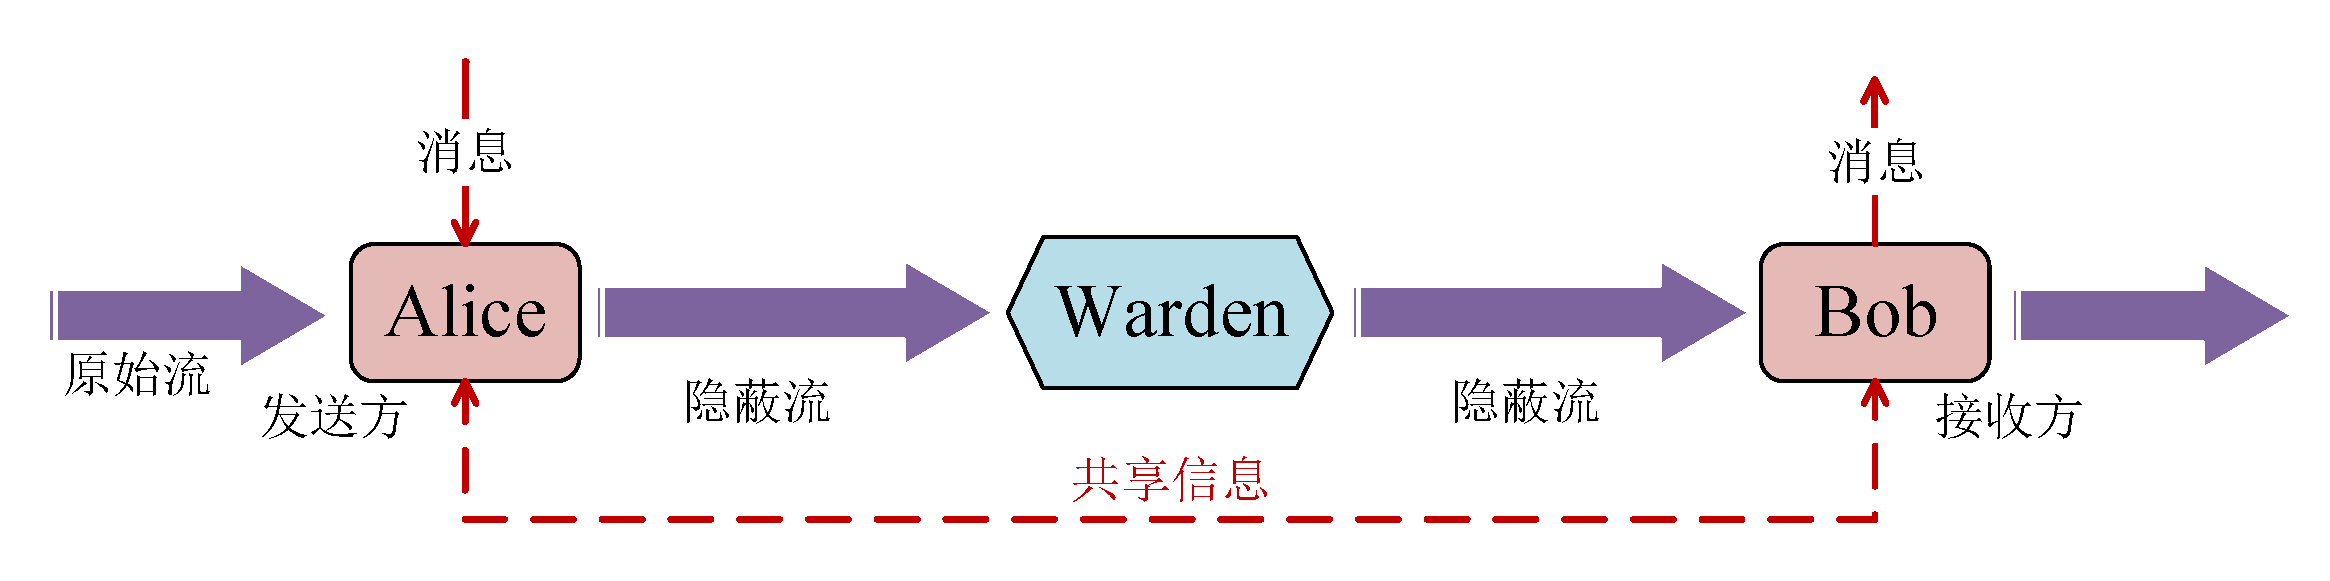
\includegraphics[width=\textwidth]{chapters/chapter1/figures/covert-channel.pdf}
        \caption{隐通道逻辑结构示意图}\label{fig:1:covert-channel}
	\end{figure}
}

对于隐通道的研究,主要集中在构建方法和检测方法两个方面。隐通道的逻辑结构示意如图\nref{fig:1:covert-channel},发送方和接收方利用共享信息,由发送方将宿主信道修改为隐蔽信道,接收方识别隐蔽信道中的特征信息,结合共享信息还原隐蔽消息。
隐通道最核心的环节,是如何实现调制过程,也就是将宿主信道修改为隐蔽信道的方式,这也是区分时间隐通道与存储隐通道的基本方法。
隐通道的检测方法,是针对特定类型的构建方法提出了,在应用范围上存在特定的局限性。
例如,基于IP(Internet Protocol)冗余字段的隐通道,修改了IP数据包头中的冗余字段,对宿主信道及上层应用不产生任何影响。对应的检测及消除措施,主要方式为扫描各字段的异常信息,并进行数据覆写,对部分存储隐通道实现有效防御。基于数据包顺序的隐通道,在构造过程中重新调整数据包序号,导致乱序现象出现,形成可检测的传输特征。通过数据包重排序,恢复正常顺序或再次打乱,在一定程度上进行消除。\nupcite{ahsan2002practical}

%时间隐通道相对存储隐通道的优势是什么
在不同的应用场景中,隐通道有多种表现形式。在单主机环境下,隐通道的构建可以利用磁盘响应时间,通过影响磁盘访问队列\nupcite{130771},实现单主机中不同进程之间的隐蔽传输;时间隐通道JitterBug捕获键盘输入中的敏感信息,并通过松耦合的网络隐通道进行传输,在SSH(Secure Shell)、VNC(Virtual Network Computing)及RDP(Remote Desktop Protocol)等远程访问场景中具有可操作性\nupcite{shah2006keyboards}。
在以太网环境中,存储隐通道的构建多基于网络协议,类似于音频、视频中常用的隐写术,待发送的消息块被嵌入到数据包中,如TCP(Transmission Control Protocol)包头中的冗余字段\nupcite{4317620}、IPv6包头中的AH及ESP字段\nupcite{10.1007/11767831_10};时间隐通道的构建,多基于数据包传输间隔及数据包发送顺序等。
相比于存储隐通道,时间隐通道在隐蔽性方面具有绝佳的优势,但受限于隐蔽信道的基础条件和网络噪声的影响,在传输能力及传输性能方面存在不足。因此,时间隐通道适用于少量核心消息的传输,存储隐通道适用于具有高性能传输需求的场景。

%移动互联网的兴起
随着第四代移动通信技术的广泛应用,以及移动智能终端的不断发展,移动互联网得到进一步发展,目前正在由4G时代过渡到5G时代\nupcite{7470940}。
第四代移动通信技术,也就是LTE(Long Term Evolution)技术,在接入带宽、空口时延及负载能力等方面均得到了提升,面向移动互联网的应用得到繁荣发展。
不同于原有的移动通信技术,LTE网络在设计中采用了全IP网络\nupcite{6398495}。网络中的所有数据均封装为IP数据包,实现了更高的数据转发能力及更低的传输延迟;对不同应用、不同类型数据包的优化及优先级调度,提供了更好的用户体验;传输网络的鲁棒性得到提升,不同应用场景下的适应能力得到提升。\nupcite{DBLP:journals/corr/abs-1810-02968}

%VoLTE是未来的趋势
由于LTE网络中取消了基于电路交换的通信技术,LTE网络中的语音通话必须向VoIP(Voice over IP)迁移,目前已经实现大规模商用。通过基于数据包交换的核心网传输方式,VoLTE在提供低延迟、高清晰度语音通话的同时,也支持低延迟的视频通话。
对于5G网络,音视频通话方案仍然会按照VoLTE的模式进行设计\nupcite{8412482},因此,对VoLTE的传输特征进行研究,并研究隐通道的存在基础及构建环境,符合技术发展趋势。
得益于LTE核心网的传输保证,VoLTE的通话质量要由于第三方VoIP方案。通过提高VoLTE数据包优先级,即使是高负载的网络环境中,通话延迟方面也具有显著优势;采用高效的编码方式,在平衡通话质量的同时,降低丢包率。\nupcite{anehill2012validating}

%研究VoLTE下时间隐通道构建方法,具有填补空白的意义
基于端到端的数据包传输,是VoLTE区别于VoIP应用的重要特征。通过减少数据包转发环节,VoLTE为时间隐通道的研究提供了新的环境,在VoLTE环境下,数据包的类型、传输顺序及网络抖动均存在较强的规律性,一定程度上破坏了时间隐通道的构建条件。研究基于主动丢包的时间隐通道方法,不仅扩充了VoLTE下隐通道的设计方法,对其它端到端传输环境也具有参考价值。
\section{国内外研究现状及难点}
\label{sec:intro:background}

本节说了什么

本节包含的内容

\subsection{基于移动互联网的时间隐通道}
\label{sec:intro:background:ctc}

在移动互联网环境下,构建时间隐通道,应当遵守怎样的约束

常用的构建方法

各种方法的总结,以及为何不能应用在VoLTE环境中

\subsection{时间隐通道的鲁棒性策略}
\label{sec:intro:background:robustness}

首先说明,时间隐通道因为自身的特性,在传输可靠性上,不如Overt Traffic

现有的时间隐通道方案,在保证鲁棒性反面,采用了怎样的手段,比如添加纠错信息、重传、特殊编码等

这些方法,对应用场景的限制及不足

\subsection{时间隐通道的检测方法}
\label{sec:intro:background:detect}

检测时间隐通道,通常从那几个要素方面进行考虑

检测判断,主要根据哪些因素来考量,包括分布、一致性

在该场景中,主要通过丢包的方法构建时间隐通道,所有,在现有的常用检测方法的基础上,还要对丢包的特征进行分析

%固定相只有物理交联结构的聚氨酯称为热塑性SMPU,而有化学交联结构称为热固性SMPU。热塑性和热固性形状记忆聚氨酯的形状记忆原理示意图如图\ref{fig:diagram}所示

%\begin{figure}
% \centering
% \includegraphics[width=0.75\textwidth]{chapters/chapter1/figures/figure1}
% \caption{热塑性形状记忆聚氨酯的形状记忆机理示意图}\label{fig:diagram}
%\end{figure}

%\begin{table}
%  \centering
%  \caption{水系聚氨酯分类} \label{tab:category}
%  \begin{tabular*}{0.9\textwidth}{@{\extracolsep{\fill}}cccc}
%  \toprule
%    类别			&水溶型		&胶体分散型		&乳液型 \\
%  \midrule
%    状态			&溶解$\sim$胶束	&分散		&白浊 \\
%    外观			&水溶型		&胶体分散型		&乳液型 \\
%    粒径$/\mu m$	&$<0.001$		&$0.001-0.1$		&$>0.1$ \\
%    重均分子量	&$1000\sim 10000$	&数千$\sim 20万$ &$>5000$ \\
%  \bottomrule
%  \end{tabular*}
%\end{table}

\section{研究内容及创新点}
\label{sec:intro:work}

\subsection{本文主要内容}
\label{sec:intro:work:mainwork}

随着VoLTE应用范围的不断扩大,研究在VoLTE环境下的时间隐通道构建方案,扩充了时间隐通道的构建方法,也进一步扩展对VoLTE音视频通话特征的研究。本文主要研究在VoLTE视频通话场景下,通过主动丢包的方式,构建鲁棒的时间隐通道。主要包括三个研究点,分别是VoLTE时间隐通道检测方法研究,基于Zigzag映射矩阵的时间隐通道构建方法研究,以及基于多重校验的时间隐通道构建方法研究。各部分之间的关联关系及研究指标如图\nref{fig:1:contents}。

\insertFigure{
	\begin{figure}
		\centering
        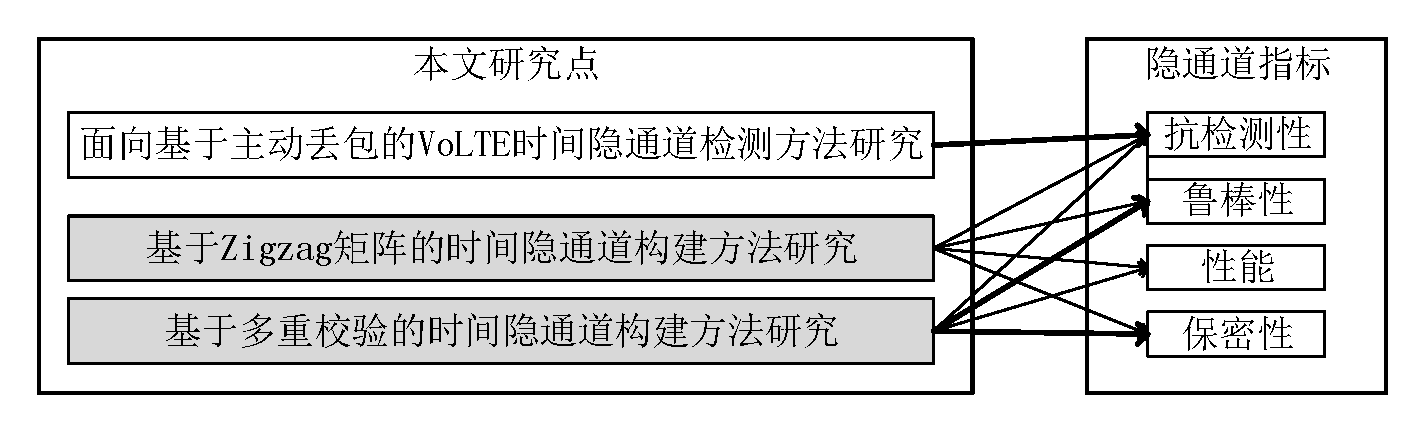
\includegraphics[width=0.75\textwidth]{chapters/chapter1/figures/struct.pdf}
        \caption{本文各研究点之间的关系}\label{fig:1:contents}
	\end{figure}
}

%背景介绍了什么
背景及相关工作部分,主要介绍了本论文主要工作的一些研究基础,以及国内外的研究现状。内容包括对VoLTE音视频传输方案的分析,分析了实际商用中VoLTE的数据产生、处理、传输、呈现流程,并分析了音视频在流程上的差异。对现有时间隐通道构造方案的分析,涵盖了以太网中的构造方案、移动互联网下的构造方案,以及有效的鲁棒性策略。通过分析VoLTE传输协议,研究丢包带来的影响,并充分利用协议中的随机字段,提高保密性。抗检测能力是时间隐通道的一个重要指标,通过研究现有的时间隐通道检测方法,针对该时间隐通道构建方法,选择可用的检测方法。

%检测方法介绍了什么
VoLTE时间隐通道检测方法研究,主要研究在VoLTE场景下,如何有效检测基于主动丢包的时间隐通道。为筛选有效的检测方法,首先对VoLTE通话抓包结果进行分析,由丢包率、IPD、突发丢包长度及丢包随机性几个方面分别展开。根据特征分析结果,提出了一组基于统计分析的时间隐通道检测方法,包含不同维度的多种检测方式。最后,通过模拟的方式,对这些方法进行模拟测试,判断是否具有显著效果。

%Zigzag方法说了什么
基于Zigzag映射矩阵的时间隐通道构建方法,研究利用Zigzag矩阵作为码字与符号关系的映射矩阵,并添加冗余校验信息,在抗检测性、鲁棒性及传输性能之间实现均衡。为了清楚地介绍该研究方法,按照研究背景、构造方法及实验结果及评估的顺序,对该方法的研究基础、架构设计、调制解调方法及实验测试结果分别进行介绍。经过实验测试证明,通过调整传输参数,该时间隐通道构建方法各方面结果良好。

%多重校验方法说了什么
基于多重校验的时间隐通道构建方法,重点研究如何进一步降低误码率,提高传输可靠性。在该时间隐通道方法中,设计了包括码字间校验、码字自校验以及符号校验三级校验模式,结合对连续丢包噪声具有抑制作用的映射矩阵,显著提高了传输鲁棒性,降低了误码率水平。该部分首先从研究背景基础开始,首先介绍该方法的设计架构,然后针对核心的鲁棒性鲁棒性方法逐层展开,最后进行实验测试与对比。实验结果表明,该时间隐通道的误码率水平较之前方案有了大幅度提升。

%以上各部分是怎样在逻辑上串起来的
背景及相关工作的介绍,分析出在VoLTE视频通话场景下,通过主动丢包的方式构建时间隐通道是可行的。与此同时,现有的检测方法及鲁棒性方法,无法有效覆盖这种隐通道构造模式。VoLTE时间隐通道检测方法研究,着重解决如何检测采用主动丢包的时间隐通道,同时也为接下来提出的构建方案提供检测依据。最后,两种不同的时间隐通道构建方法,分别从不同的方式,填补鲁棒性方面的构建需求,并通过实验进行验证。

\subsection{本文主要创新点}
\label{sec:intro:work:inno}

本文的研究重点,是在VoLTE场景下,通过主动丢包方式构建时间隐通道的方法,以及抗检测性评估方式。主要的创新点包括以下几点:

\begin{enumerate}
    \item 提出了一种VoLTE下时间隐通道检测方法,针对基于主动丢包的构建方法。该方法以统计分析为基础,综合多种量化评估方法,结合IPD及丢包特征两个维度进行检测判别。传统的时间隐通道检测方法,主要基于IPD分布特征进行检测识别,对基于主动丢包的时间隐通道来说,判别效果不够全面。本方法完善了时间隐通道的检测方式,经过实验测试,该时间隐通道检测方法有效可行。
    \item 提出了一种基于Zigzag映射矩阵的时间隐通道构建方法,该方法的核心,是隐通道的编码及调制过程,在编码过程中添加CRC校验信息,利用Zigzag矩阵完成码字到符号的转换,最后添加随机偏移量得到要丢弃的数据包序号。该方法以简单高效的方式,以轻量级校验模式,在保证传输性能的同时,降低计算复杂度保证鲁棒性,适用于容许一定误码率的应用场景。
    \item 提出了一种基于多重校验的时间隐通道构造方法,重点研究如何通过逐级校验的方式,降低噪声对时间隐通道的干扰,提高噪声干扰下的鲁棒性。该方法的核心,是在不同的处理阶段引入相互独立的校验方式,在解调过程中逐级剔除噪声干扰,还原概率最高的隐蔽消息。此外,通过引入可调映射矩阵,将连续丢包事件分散到多个组,减小每组的噪声强度,降低误码率水平。
\end{enumerate}

\subsection{本文组织结构}
\label{sec:intro:work:struct}

全文共分五章,文章的组织结构如下:
\begin{itemize}
    \item 第1章,对本文的研究领域及主要内容进行介绍
    \item 第2章,本文中涉及到的研究背景,及国内外相关工作的介绍。包含当前研究工作的基础介绍,当前隐通道构建及检测方面的研究成果,以及时间隐通道应当满足的基本要求。
    \item 第3章,介绍VoLTE下时间隐通道检测方法,结合当前成熟的检测方法,在IPD检测的基础上,添加对丢包特征统计的检测。监测维度涵盖了基于统计曲线的检测、基于熵的检测及基于相对距离的检测方法,能够对基于主动丢包的时间隐通道进行有效识别。该检测方法,也是本文两种时间隐通道构建方法抗检测能力的评估参照。
    \item 第4章,介绍基于Zigzag映射矩阵的时间隐通道构建方法,由研究背景开始,首先介绍构建方法的设计方案,然后通过实验,对隐通道的各项指标进行评估。
    \item 第5章,介绍基于多重校验的时间隐通道构建方法,首先对方法背景进行介绍,然后对时间隐通道的整体流程进行展开,接下来对关键的鲁棒性方案设计逐级展开分析,最后分析实验结果及指标。
\end{itemize}

%%%%%%%%%%%%%论文正文部分%%%%%%%%%%%%%%%%%%%%%%%%%%%%%%%%%%%%%%%%
\chapter{引言}
\label{chap:intro}
%在下方加入各小节内容
\section{研究背景和意义}
\label{sec:intro:backgroud}

%介绍什么是隐通道

%传统的时间隐通道,是利用数据的时间变化特性,承载目标数据。例如基于IP的时间隐通道(IP-CTC)[3].,基于回复时间的隐通道(TR-CTC)[4].,基于IPD的时间隐通道(IPD-CTC),利用数据包的长度变化规律来传送数据[10].,利用数据包之间的时间间隔(IPD)传送数据[12].,或者基于数据包分类的时间隐通道[13].,以及基于模型的时间隐通道(MB-CTC)[11].。

隐通道的明确定义,由Lampson在1973年提出\nupcite{4317620},隐通道能够打破系统中的安全限制,实现消息在不同安全级别之间的隐蔽传输。隐通道的存在意义,是在传输信道被监听的前提下,实现数据传输过程,并且监听者无法察觉传输过程。监听者通常对数据内容及传输过程进行监控,只允许传输符合规则的数据,拦截其它的会话请求。研究VoLTE中的时间隐通道构建方法,解决当双方只被允许进行VoLTE通话时,数据隐蔽、鲁棒传输的需求。

经过研究探索,随着互联网应用范围的扩大,网络应用逐渐丰富,隐通道的应用环境由传统的单主机平台,扩展到各种类型的网络设备之中。
隐通道的实现方式多种多样,根据构建方式的差异,隐通道通常被划分为时间隐通道及存储隐通道两种类型,存储隐通道依赖于双方对相同存储位置的读写访问,时间隐通道依赖于双方对时间特征的识别。\nupcite{1702197}
随着移动互联网的不断扩展,隐通道为终端之间的安全隐蔽传输,提供了可行的解决方案,满足了特定需求场景下的传输需求。\nupcite{6542541}

\insertFigure{
	\begin{figure}
	    \centering
        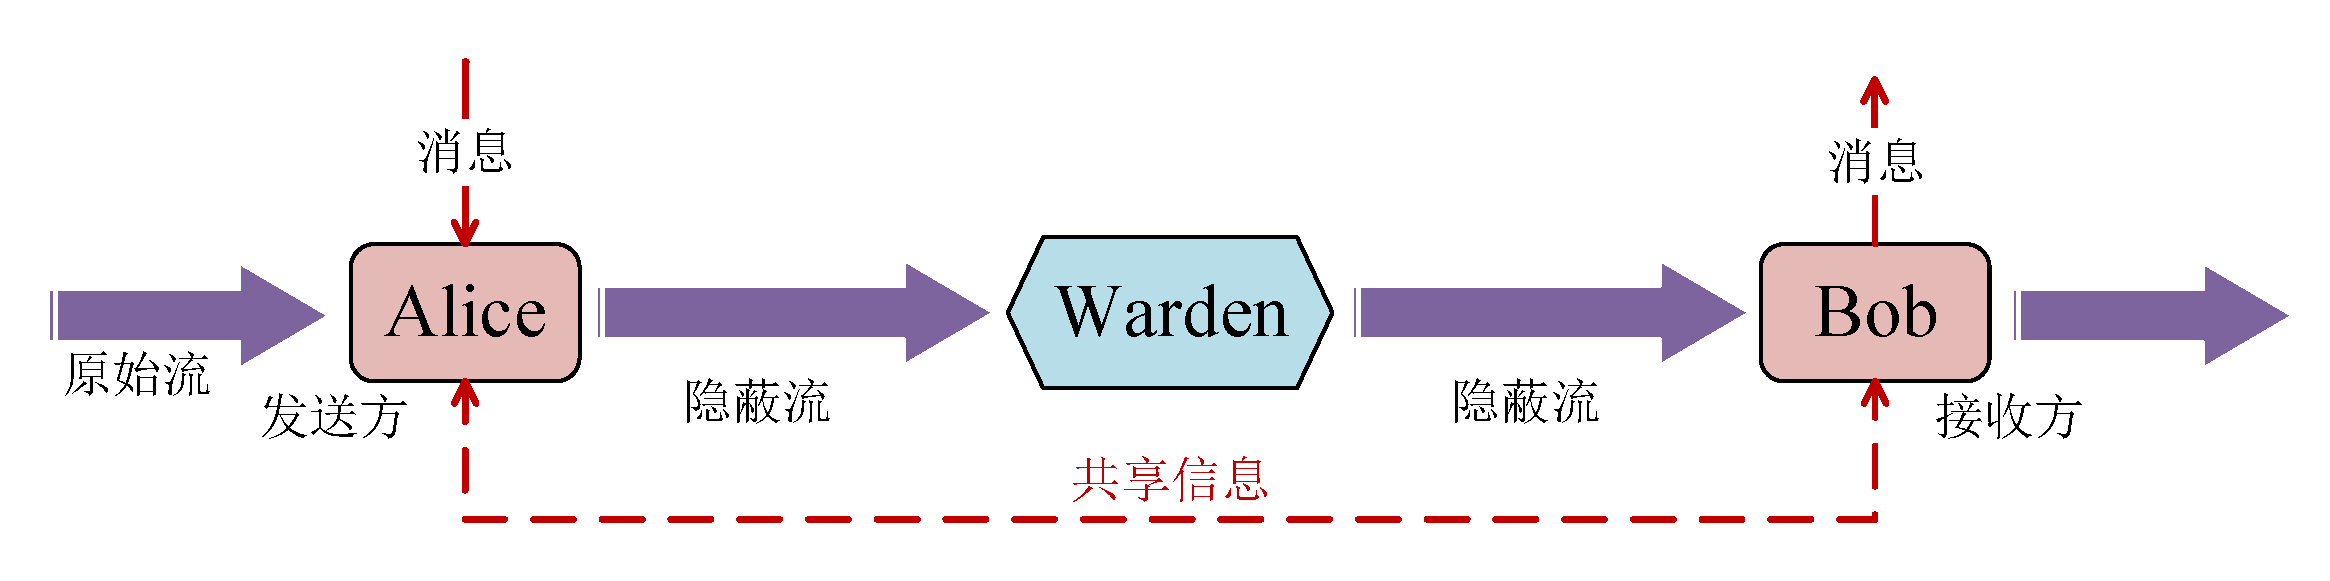
\includegraphics[width=\textwidth]{chapters/chapter1/figures/covert-channel.pdf}
        \caption{隐通道逻辑结构示意图}\label{fig:1:covert-channel}
	\end{figure}
}

对于隐通道的研究,主要集中在构建方法和检测方法两个方面。隐通道的逻辑结构示意如图\nref{fig:1:covert-channel},发送方和接收方利用共享信息,由发送方将宿主信道修改为隐蔽信道,接收方识别隐蔽信道中的特征信息,结合共享信息还原隐蔽消息。
隐通道最核心的环节,是如何实现调制过程,也就是将宿主信道修改为隐蔽信道的方式,这也是区分时间隐通道与存储隐通道的基本方法。
隐通道的检测方法,是针对特定类型的构建方法提出了,在应用范围上存在特定的局限性。
例如,基于IP(Internet Protocol)冗余字段的隐通道,修改了IP数据包头中的冗余字段,对宿主信道及上层应用不产生任何影响。对应的检测及消除措施,主要方式为扫描各字段的异常信息,并进行数据覆写,对部分存储隐通道实现有效防御。基于数据包顺序的隐通道,在构造过程中重新调整数据包序号,导致乱序现象出现,形成可检测的传输特征。通过数据包重排序,恢复正常顺序或再次打乱,在一定程度上进行消除。\nupcite{ahsan2002practical}

%时间隐通道相对存储隐通道的优势是什么
在不同的应用场景中,隐通道有多种表现形式。在单主机环境下,隐通道的构建可以利用磁盘响应时间,通过影响磁盘访问队列\nupcite{130771},实现单主机中不同进程之间的隐蔽传输;时间隐通道JitterBug捕获键盘输入中的敏感信息,并通过松耦合的网络隐通道进行传输,在SSH(Secure Shell)、VNC(Virtual Network Computing)及RDP(Remote Desktop Protocol)等远程访问场景中具有可操作性\nupcite{shah2006keyboards}。
在以太网环境中,存储隐通道的构建多基于网络协议,类似于音频、视频中常用的隐写术,待发送的消息块被嵌入到数据包中,如TCP(Transmission Control Protocol)包头中的冗余字段\nupcite{4317620}、IPv6包头中的AH及ESP字段\nupcite{10.1007/11767831_10};时间隐通道的构建,多基于数据包传输间隔及数据包发送顺序等。
相比于存储隐通道,时间隐通道在隐蔽性方面具有绝佳的优势,但受限于隐蔽信道的基础条件和网络噪声的影响,在传输能力及传输性能方面存在不足。因此,时间隐通道适用于少量核心消息的传输,存储隐通道适用于具有高性能传输需求的场景。

%移动互联网的兴起
随着第四代移动通信技术的广泛应用,以及移动智能终端的不断发展,移动互联网得到进一步发展,目前正在由4G时代过渡到5G时代\nupcite{7470940}。
第四代移动通信技术,也就是LTE(Long Term Evolution)技术,在接入带宽、空口时延及负载能力等方面均得到了提升,面向移动互联网的应用得到繁荣发展。
不同于原有的移动通信技术,LTE网络在设计中采用了全IP网络\nupcite{6398495}。网络中的所有数据均封装为IP数据包,实现了更高的数据转发能力及更低的传输延迟;对不同应用、不同类型数据包的优化及优先级调度,提供了更好的用户体验;传输网络的鲁棒性得到提升,不同应用场景下的适应能力得到提升。\nupcite{DBLP:journals/corr/abs-1810-02968}

%VoLTE是未来的趋势
由于LTE网络中取消了基于电路交换的通信技术,LTE网络中的语音通话必须向VoIP(Voice over IP)迁移,目前已经实现大规模商用。通过基于数据包交换的核心网传输方式,VoLTE在提供低延迟、高清晰度语音通话的同时,也支持低延迟的视频通话。
对于5G网络,音视频通话方案仍然会按照VoLTE的模式进行设计\nupcite{8412482},因此,对VoLTE的传输特征进行研究,并研究隐通道的存在基础及构建环境,符合技术发展趋势。
得益于LTE核心网的传输保证,VoLTE的通话质量要由于第三方VoIP方案。通过提高VoLTE数据包优先级,即使是高负载的网络环境中,通话延迟方面也具有显著优势;采用高效的编码方式,在平衡通话质量的同时,降低丢包率。\nupcite{anehill2012validating}

%研究VoLTE下时间隐通道构建方法,具有填补空白的意义
基于端到端的数据包传输,是VoLTE区别于VoIP应用的重要特征。通过减少数据包转发环节,VoLTE为时间隐通道的研究提供了新的环境,在VoLTE环境下,数据包的类型、传输顺序及网络抖动均存在较强的规律性,一定程度上破坏了时间隐通道的构建条件。研究基于主动丢包的时间隐通道方法,不仅扩充了VoLTE下隐通道的设计方法,对其它端到端传输环境也具有参考价值。
\section{国内外研究现状及难点}
\label{sec:intro:background}

本节说了什么

本节包含的内容

\subsection{基于移动互联网的时间隐通道}
\label{sec:intro:background:ctc}

在移动互联网环境下,构建时间隐通道,应当遵守怎样的约束

常用的构建方法

各种方法的总结,以及为何不能应用在VoLTE环境中

\subsection{时间隐通道的鲁棒性策略}
\label{sec:intro:background:robustness}

首先说明,时间隐通道因为自身的特性,在传输可靠性上,不如Overt Traffic

现有的时间隐通道方案,在保证鲁棒性反面,采用了怎样的手段,比如添加纠错信息、重传、特殊编码等

这些方法,对应用场景的限制及不足

\subsection{时间隐通道的检测方法}
\label{sec:intro:background:detect}

检测时间隐通道,通常从那几个要素方面进行考虑

检测判断,主要根据哪些因素来考量,包括分布、一致性

在该场景中,主要通过丢包的方法构建时间隐通道,所有,在现有的常用检测方法的基础上,还要对丢包的特征进行分析

%固定相只有物理交联结构的聚氨酯称为热塑性SMPU,而有化学交联结构称为热固性SMPU。热塑性和热固性形状记忆聚氨酯的形状记忆原理示意图如图\ref{fig:diagram}所示

%\begin{figure}
% \centering
% \includegraphics[width=0.75\textwidth]{chapters/chapter1/figures/figure1}
% \caption{热塑性形状记忆聚氨酯的形状记忆机理示意图}\label{fig:diagram}
%\end{figure}

%\begin{table}
%  \centering
%  \caption{水系聚氨酯分类} \label{tab:category}
%  \begin{tabular*}{0.9\textwidth}{@{\extracolsep{\fill}}cccc}
%  \toprule
%    类别			&水溶型		&胶体分散型		&乳液型 \\
%  \midrule
%    状态			&溶解$\sim$胶束	&分散		&白浊 \\
%    外观			&水溶型		&胶体分散型		&乳液型 \\
%    粒径$/\mu m$	&$<0.001$		&$0.001-0.1$		&$>0.1$ \\
%    重均分子量	&$1000\sim 10000$	&数千$\sim 20万$ &$>5000$ \\
%  \bottomrule
%  \end{tabular*}
%\end{table}

\section{研究内容及创新点}
\label{sec:intro:work}

\subsection{本文主要内容}
\label{sec:intro:work:mainwork}

随着VoLTE应用范围的不断扩大,研究在VoLTE环境下的时间隐通道构建方案,扩充了时间隐通道的构建方法,也进一步扩展对VoLTE音视频通话特征的研究。本文主要研究在VoLTE视频通话场景下,通过主动丢包的方式,构建鲁棒的时间隐通道。主要包括三个研究点,分别是VoLTE时间隐通道检测方法研究,基于Zigzag映射矩阵的时间隐通道构建方法研究,以及基于多重校验的时间隐通道构建方法研究。各部分之间的关联关系及研究指标如图\nref{fig:1:contents}。

\insertFigure{
	\begin{figure}
		\centering
        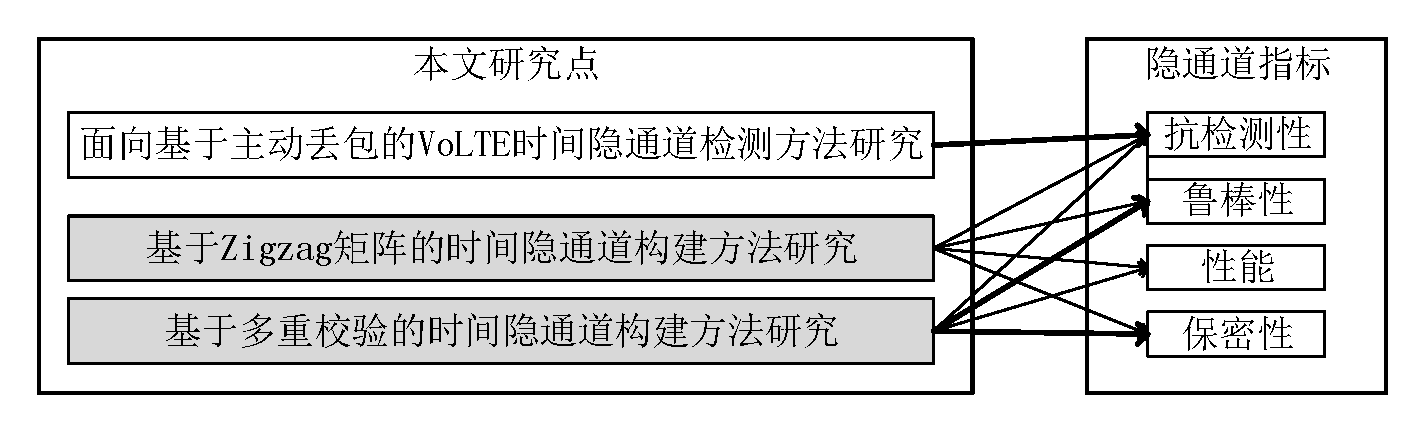
\includegraphics[width=0.75\textwidth]{chapters/chapter1/figures/struct.pdf}
        \caption{本文各研究点之间的关系}\label{fig:1:contents}
	\end{figure}
}

%背景介绍了什么
背景及相关工作部分,主要介绍了本论文主要工作的一些研究基础,以及国内外的研究现状。内容包括对VoLTE音视频传输方案的分析,分析了实际商用中VoLTE的数据产生、处理、传输、呈现流程,并分析了音视频在流程上的差异。对现有时间隐通道构造方案的分析,涵盖了以太网中的构造方案、移动互联网下的构造方案,以及有效的鲁棒性策略。通过分析VoLTE传输协议,研究丢包带来的影响,并充分利用协议中的随机字段,提高保密性。抗检测能力是时间隐通道的一个重要指标,通过研究现有的时间隐通道检测方法,针对该时间隐通道构建方法,选择可用的检测方法。

%检测方法介绍了什么
VoLTE时间隐通道检测方法研究,主要研究在VoLTE场景下,如何有效检测基于主动丢包的时间隐通道。为筛选有效的检测方法,首先对VoLTE通话抓包结果进行分析,由丢包率、IPD、突发丢包长度及丢包随机性几个方面分别展开。根据特征分析结果,提出了一组基于统计分析的时间隐通道检测方法,包含不同维度的多种检测方式。最后,通过模拟的方式,对这些方法进行模拟测试,判断是否具有显著效果。

%Zigzag方法说了什么
基于Zigzag映射矩阵的时间隐通道构建方法,研究利用Zigzag矩阵作为码字与符号关系的映射矩阵,并添加冗余校验信息,在抗检测性、鲁棒性及传输性能之间实现均衡。为了清楚地介绍该研究方法,按照研究背景、构造方法及实验结果及评估的顺序,对该方法的研究基础、架构设计、调制解调方法及实验测试结果分别进行介绍。经过实验测试证明,通过调整传输参数,该时间隐通道构建方法各方面结果良好。

%多重校验方法说了什么
基于多重校验的时间隐通道构建方法,重点研究如何进一步降低误码率,提高传输可靠性。在该时间隐通道方法中,设计了包括码字间校验、码字自校验以及符号校验三级校验模式,结合对连续丢包噪声具有抑制作用的映射矩阵,显著提高了传输鲁棒性,降低了误码率水平。该部分首先从研究背景基础开始,首先介绍该方法的设计架构,然后针对核心的鲁棒性鲁棒性方法逐层展开,最后进行实验测试与对比。实验结果表明,该时间隐通道的误码率水平较之前方案有了大幅度提升。

%以上各部分是怎样在逻辑上串起来的
背景及相关工作的介绍,分析出在VoLTE视频通话场景下,通过主动丢包的方式构建时间隐通道是可行的。与此同时,现有的检测方法及鲁棒性方法,无法有效覆盖这种隐通道构造模式。VoLTE时间隐通道检测方法研究,着重解决如何检测采用主动丢包的时间隐通道,同时也为接下来提出的构建方案提供检测依据。最后,两种不同的时间隐通道构建方法,分别从不同的方式,填补鲁棒性方面的构建需求,并通过实验进行验证。

\subsection{本文主要创新点}
\label{sec:intro:work:inno}

本文的研究重点,是在VoLTE场景下,通过主动丢包方式构建时间隐通道的方法,以及抗检测性评估方式。主要的创新点包括以下几点:

\begin{enumerate}
    \item 提出了一种VoLTE下时间隐通道检测方法,针对基于主动丢包的构建方法。该方法以统计分析为基础,综合多种量化评估方法,结合IPD及丢包特征两个维度进行检测判别。传统的时间隐通道检测方法,主要基于IPD分布特征进行检测识别,对基于主动丢包的时间隐通道来说,判别效果不够全面。本方法完善了时间隐通道的检测方式,经过实验测试,该时间隐通道检测方法有效可行。
    \item 提出了一种基于Zigzag映射矩阵的时间隐通道构建方法,该方法的核心,是隐通道的编码及调制过程,在编码过程中添加CRC校验信息,利用Zigzag矩阵完成码字到符号的转换,最后添加随机偏移量得到要丢弃的数据包序号。该方法以简单高效的方式,以轻量级校验模式,在保证传输性能的同时,降低计算复杂度保证鲁棒性,适用于容许一定误码率的应用场景。
    \item 提出了一种基于多重校验的时间隐通道构造方法,重点研究如何通过逐级校验的方式,降低噪声对时间隐通道的干扰,提高噪声干扰下的鲁棒性。该方法的核心,是在不同的处理阶段引入相互独立的校验方式,在解调过程中逐级剔除噪声干扰,还原概率最高的隐蔽消息。此外,通过引入可调映射矩阵,将连续丢包事件分散到多个组,减小每组的噪声强度,降低误码率水平。
\end{enumerate}

\subsection{本文组织结构}
\label{sec:intro:work:struct}

全文共分五章,文章的组织结构如下:
\begin{itemize}
    \item 第1章,对本文的研究领域及主要内容进行介绍
    \item 第2章,本文中涉及到的研究背景,及国内外相关工作的介绍。包含当前研究工作的基础介绍,当前隐通道构建及检测方面的研究成果,以及时间隐通道应当满足的基本要求。
    \item 第3章,介绍VoLTE下时间隐通道检测方法,结合当前成熟的检测方法,在IPD检测的基础上,添加对丢包特征统计的检测。监测维度涵盖了基于统计曲线的检测、基于熵的检测及基于相对距离的检测方法,能够对基于主动丢包的时间隐通道进行有效识别。该检测方法,也是本文两种时间隐通道构建方法抗检测能力的评估参照。
    \item 第4章,介绍基于Zigzag映射矩阵的时间隐通道构建方法,由研究背景开始,首先介绍构建方法的设计方案,然后通过实验,对隐通道的各项指标进行评估。
    \item 第5章,介绍基于多重校验的时间隐通道构建方法,首先对方法背景进行介绍,然后对时间隐通道的整体流程进行展开,接下来对关键的鲁棒性方案设计逐级展开分析,最后分析实验结果及指标。
\end{itemize}
%%%%%%%%%%%%以下部分仅用于举例样式%%%%%%%%%%%%%%%%%%%%%%%%%%%%%%%
\chapter{部分新增命令使用示例}
\fbox{自查重模式下使用$\backslash$insert*系列命令指定的内容将不被显示。}\\
\begin{lstlisting}[language={tex}, caption={$\backslash$insert*系列指令使用示例}]
\insertContents{
	anything contents....
}
\insertFigure{
	\begin{figure}
		.......
	\end{figure}
}
\insertTable{
	\begin{table}
		.......
	\end{table}
}
\insertEquation{
	\begin{equation}
		......
	\end{equation}
}
\end{lstlisting}
%结论

自查重模式下使用$\backslash$ncite、$\backslash$nupcite、$\backslash$nref命令进行的引用,引用标注将不显示。使用方式同$\backslash$cite、$\backslash$upcite、$\backslash$ref。

\begin{conclusion}

本文主要研究在VoLTE中通过主动丢包方式构建时间隐通道,主要研究要点包括VoLTE主动丢包时间隐通道的检测方法、基于Zigzag映射矩阵的时间隐通道构建方法、基于多重校验纠错的时间隐通道构建方法,以及基于Linphone的时间隐通道原型系统。其中,VoLTE主动丢包时间隐通道的检测方法,提出了检测基于主动丢包时间隐通道的方法,有助于提升时间隐通道的构建水平。基于Zigzag映射矩阵的时间隐通道构建方法,以及基于多重校验纠错的时间隐通道构建方法,提出了两种基于主动丢包的时间隐通道构建方法,在抗检测能力、鲁棒性、传输性能及构建代价方面均具有良好测试结果。基于Linphone的时间隐通道原型系统,借助Linphone与VoLTE相同的SIP+RTP传输模式,验证通过主动丢包构建时间隐通道的可行性,并进行实际传输测试验证其有效性。

本文主要研究内容及创新点总结如下:
\begin{enumerate}
    \item
    提出了一种VoLTE主动丢包时间隐通道的检测方法,完善了VoLTE环境中的时间隐通道检测方法,有助于提高时间隐通道构建水平。当前的时间隐通道检测方法,多针对IPD分布特征。然而,基于主动丢包的时间隐通道对IPD分布影响有限,常规检测方法准确率较低。因此,本方法除了统计IPD分布外,同时考虑了连续丢包数分布及区间丢包数分布。为有效检测统计分布之间的差异,除了常用的CDF检测、K-S检验及K-L散度检验,本方法中同时参考Welch's t检验、Mann–Whitney rank检验、Wasserstein距离以及能量距离的测试结果。并约定只有通过了所有的检测子项,才认定不存在时间隐通道。
    
    基于模拟的时间隐通道进行检测能力测试,该时间隐通道的测试效果达到了设计要求。VoLTE通话的Excellent场景中,当主动丢包率不低于{0.4\ \%}时,该方法具有{100\ \%}检出能力;VoLTE通话的Good场景中,当主动丢包率不低于{1\ \%}时,该方法具有{100\ \%}检出能力。作为对比,仅采用基于IPD的检测方法时,主动丢包率低于{2\ \%}即可通过常用的K-S检验及K-L散度检验,证明该检测方法在检测能力方面有了较大提升。
    
    \item
    提出了基于Zigzag映射矩阵的时间隐通道构建方法,同时满足了抗检测能力、鲁棒性、传输性能及保密性方面的设计指标。该方法中,主要的参数为码字长度$L_{Codeword}$,通过调整码字长度在各指标方面实现均衡。该方法的调制过程主要包括三个流程,分别为消息分组、校验码字生成以及码字-符号映射;解调过程中对应为消息重组、有效码字鉴别以及符号-码字逆映射。其中,消息分组过程按照设定的码字长度,将隐蔽消息切分为等长消息块,解调过程按照顺序进行重组。
    
    为保证时间隐通道的鲁棒性,在消息块的基础上,计算每一个消息块对应的CRC校验值,作为校验码字插入到码字集合中。解调过程中,借助CRC的确定性鉴别码字与噪声,在一定程度上去除噪声干扰。Zigzag矩阵作用于符号与码字之间的转换,消除了符号与码字间的线性关系。通过映射矩阵随机初始化,有效提高了时间隐通道的保密性。经过实验测试,该方法具有良好的抗检测能力,并且传输性能达到{0.88\ bps}时误码率在{1.5\ \%}左右,同时具有较小的构建代价。
    
    \item
    提出了基于多重校验纠错的时间隐通道构建方法,重点提升时间隐通道的鲁棒性,降低传输误码率。基于主动丢包的时间隐通道虽然具有良好的隐蔽性,但信号与噪声相似度较高,具有较低的信噪比,单一的数据校验与纠错无法满足实际需求。本方法的校验纠错包含三部分,分别为基于HASH的码字间校验方法、基于CRC的码字自校验方法以及基于异或的映射矩阵校验方法。其中,基于HASH的码字间校验方法建立了码字间的关联关系,利用后接收的码字验证已接收的码字。基于CRC的码字自校验,降低了编码密度,有效过滤噪声。基于异或的映射矩阵校验,通过码字-符号转换过程的校验符号,在符号层面进行预先校验。
    
    解调过程中,逐层检验校验信息,通过每一重校验进行纠错,提高了时间隐通道的鲁棒性。此外,计算校验信息时,通过引入随机信息及共享信息,提高了时间隐通道的随机性与保密性。经实验测试,该方法在传输速率达到{0.49\ bps}时,误码率不高于{0.08\ \%},鲁棒性得到提升。同时在构建代价方面,通过视频质量的客观评估指标评测,该方法产生的影响小于网络噪声的影响。

    \item
    Linphone平台中,搭建了基于主动丢包的时间隐通道原型系统。通过在Linphone中添加隐通道控制接口、隐通道传输接口及隐通道执行组件,提供了UI层时间隐通道控制命令,实现了隐蔽消息通过主动丢包序号传送。借助Linphone与VoLTE在传输模式上的相似性,测试证明了基于主动丢包的时间隐通道具有可行性。根据不同网络环境下的测试结果,原型系统符合SIP+RTP的传输模式,并且对应用及通话质量具有较小影响。
\end{enumerate}

一系列实验证明,基于主动丢包的时间隐通道构建方法,抗检测能力方面能够通过严苛的统计检验,实际测试中具有良好的可用性。结合本文中提出的时间隐通道构建方法,能够有效提升鲁棒性,并且传输性能达到时间隐通道的基本水平。保密性方面,结合RTP包头中的随机字段,实现处理过程中的加盐及随机化,增强了传输过程的随机性。基于主动丢包的时间隐通道,在保证隐蔽性的前提下具有较低的主动丢包率。因此,本文中时间隐通道对用户体验及通话质量的影响有限,并且低于网络噪声产生的波动,构建代价影响较小。

当前,基于主动丢包的时间隐通道已经具备良好的理论基础,并且通过了原型系统测试。但实际应用环境复杂且动态变化,时间隐通道需要一定的环境适应能力,才能充分利用信道资源,在保证数据完整性的基础上提高性能。因此,在以下几个方向仍然具有研究意义:
\begin{enumerate}
    \item
    时间隐通道与网络环境自适应,实现传输参数动态调整。实验测试表明,不同网络环境的特征存在差异,网络噪声水平也不尽相同。隐通道的目标,是在保持隐蔽性的前提下,以较高的质量传输更多的数据。因此,在传输过程中进行网络质量评估,调整传输参数使其与网络环境相适应,能够挖掘传输潜力,在一定程度上提升隐通道指标。
    
    \item
    会话协商及传输确认,确保隐蔽消息完整性。VoLTE通话场景中,时间隐通道具备双向传输能力,隐蔽消息接收方能够反馈传输状态。可靠性传输中,通常采用数据校验及传输确认的方式,确保接收方得到的消息完整无误。研究在时间隐通道中添加传输控制,在低误码率的基础上,将可靠度提升到{100\ \%}是有意义的研究方向。但要实现完全可靠,隐通道的传输性能将受到影响,存在一定的局限性。
    
    \item
    VoLTE场景中部署及测试,实现时间隐通道应用化。虽然VoIP与VoLTE传输模式类似,但网络环境及传输稳定性方面弱于VoLTE,尤其是视频通话的稳定性及通话延迟方面。随着5G商用规模的扩大,基于5G的音视频通话也会采用类似的模式,因此该类时间隐通道具有较长的生命周期。另一方面,即使音视频通话采用SRTP(Secure Real-time Transport Protocol)或DTLS(Datagram Transport Layer Security)进行数据加密,基于主动丢包的时间隐通道依然可行。因此,VoLTE中时间隐通道应用化,在当前及未来的网络场景中均具有应用价值。

\end{enumerate}

\end{conclusion}
%%%%%%%%%%%%%%%%%%%%%%%%%%%%%%%%%%%%%%%%%%%%%%%%%%%%%%%%%%%%%%%%%

%%%%%%%%%%%%%%%%%%%%%%%%%%%%%%%%%%%%%%%%%%%%%%%%%%%%%%%%%%%%%%%%%
%% 参考文献,五号字,使用 BibTeX,包含参考文献文件.bib
%\bibliography{reference/chap1,reference/chap2} %多个章节的参考文献
\bibliography{reference/references}


%%%%%%%%%%%%%%%%%%%%%%%%%%%%%%
%% 后置部分
%%%%%%%%%%%%%%%%%%%%%%%%%%%%%%

%% 附录(章节编号重新计算,使用字母进行编号)
\appendix
\renewcommand\theequation{\Alph{chapter}--\arabic{equation}}  % 附录中编号形式是"A-1"的样子
\renewcommand\thefigure{\Alph{chapter}--\arabic{figure}}
\renewcommand\thetable{\Alph{chapter}--\arabic{table}}

\include{chapters/app1} 
\include{chapters/app2} 

%(其后部分无编号)
\backmatter

% 发表文章目录

%% 如果只有论文成果,采用默认模式
%\begin{publications}{99}
   %\pubitem{二}{一}{Yu-an Tan, Xinting Xu, Chen Liang, Xiaosong Zhang, Quanxin Zhang and Yuanzhang Li}{An end-to-end covert channel via packet dropout for mobile networks}{J}{International Journal of Distributed Sensor Networks, 2018, 14(5), 1-14.(SCI期刊)}
   %% 盲审状态下显示:第二作者,导师第一作者+ An end-to-end covert channel via packet dropout formobile networks + International Journal of Distributed Sensor Networks, 2018, 14(5),1-14.(SCI期刊).
   %% 正常状态下显示:第二作者,导师第一作者. Yu-an Tan, Xinting Xu, Chen Liang, Xiaosong Zhang,Quanxin Zhang and Yuanzhang Li. An end-to-end covert channel via packet dropoutfor mobile networks[J]. International Journal of Distributed Sensor Networks, 2018,14(5), 1-14.(SCI期刊).
%\end{publications}
%% 默认论文成果结束

%% pubitem参数类型
%% {学生作者顺序}{老师作者顺序}{作者列表}{论文题目}{论文类型}{期刊或会议信息}
%% end

%% pubitemOthers参数类型
%% {学生作者顺序}{作者列表}{论文题目}{论文类型}{期刊或会议信息}
%% end

%% patentitem参数类型
%% {学生发明人顺序}{导师发明人顺序}{专利申请人}{专利名称}{专利申请号}{专利公开号}{专利公开时间}
%% end

%% projectitem参数类型
%% {项目类型}{项目名称}{起止时间}
%% end

%% XuXinting 添加的学术成果模式,包含三个部分:发表论文、申请专利和参与项目
%% 章标题只在researchsummary部分出现,每部分添加小标题

%% 发表论文列表
\begin{researchsummary}{99}
    \pubitem{二}{一}{Yu-an Tan, \textbf{Xinting Xu}, Chen Liang, Xiaosong Zhang, Quanxin Zhang and Yuanzhang Li}{An end-to-end covert channel via packet dropout for mobile networks}{J}{International Journal of Distributed Sensor Networks, 2018, 14(5), 1-14. (SCI期刊)}

    \pubitemOthers{三}{Yuanzhang Li, Xiaosong Zhang, \textbf{Xinting Xu}, Yu-an Tan}{A Robust Packet-Dropout Covert Channel over Wireless Networks}{J}{IEEE Wireless Communications, 2020, 27(3), 60-65. (SCI期刊)}

\end{researchsummary}

%% 申请专利列表,不需要可删
\begin{researchpatents}{99}
    \patentitem{二}{一}{谭毓安,\textbf{徐欣廷},杨恺,姜宏伟,王坤庆}{一种基于主动丢包的时间隐通道鲁棒构建方法(发明专利)}{ZL201910648138.5}{(已授权)}
\end{researchpatents}

%% 参与项目列表,不需要可删
\begin{researchprojects}{99}
    \projectitem{国家自然科学基金联合基金重点项目}{面向移动互联网实时交互应用的时间隐通道(U1636213)}{2017.01-2020.12}
\end{researchprojects}

% 致谢
%%==================================================
%% thanks.tex for BIT Master Thesis
%% modified by yang yating
%% version: 0.1
%% last update: Dec 25th, 2016
%%==================================================

%\begin{thanks}
%这个是官方模板的做法
%本论文的工作是在导师……。
%\end{thanks}

\sayThanks{
%这是模板BIT-thesis-template-grd-jdh中新增的命令,用以实现在盲审模式下关闭这一部分的显示
%注意是使用BIT-thesis-grd-jdh.cls格式控制文件的情况下
感谢人民,感谢党。

}

% 作者简介(博士论文需要)
\include{chapters/resume}


\end{document}
